\documentclass{article} % loại tài liệu
\usepackage[utf8]{vietnam} % tiếng Việt
\usepackage[left = 3.5cm,right = 2cm,top = 3.5cm,bottom = 3cm]{geometry} % căn lề
\usepackage{tikz} % vẽ hình
\usetikzlibrary{calc} % tính toán vẽ hình
\usepackage{graphicx} % hình ảnh
\usepackage{pdfpages} % thêm file pdf bao_cao_tien_do
\begin{document} % bắt đầu
%%%%%%%%%%%%%%%%%%%%%%%%%%%%%%%%%%%%%
% \begin{titlepage}
\begin{tikzpicture}[remember picture, overlay]
\draw [line width = 3pt]
($ (current page.north west) + (3.0cm, - 2.5cm)$)
rectangle
($ (current page.south east) + (- 2.5cm, 2.5cm)$);
\draw [line width = 0.5pt]
($ (current page.north west) + (3.1cm, - 2.6cm)$)
rectangle
($ (current page.south east) + (- 2.6cm, 2.6cm)$);
\end{tikzpicture}
\begin{center}
\vspace{- 0.4cm}
\textbf{ĐẠI HỌC BÁCH KHOA HÀ NỘI} \\
\textbf{VIỆN TOÁN ỨNG DỤNG VÀ TIN HỌC} \\
\textbf{******}
\vspace{0.8cm}

\begin{figure}[h]
\centering

\includegraphics[scale = .5]{pictures/logoBK.png}
\end{figure}
\vspace{0.7cm}
\textbf{\fontsize{16pt}{30pt}\selectfont {BÁO CÁO ĐỒ ÁN II}} \\
\vspace{1cm}
\textbf{\fontsize{20pt}{24pt}\selectfont {ĐỀ TÀI:}} \\
\textbf{\fontsize{19pt}{24pt}\selectfont {Xây dựng kiến trúc vi dịch vụ cho bài toán hóa đơn điện tử}} \\
% \textbf{\fontsize{20pt}{24pt}\selectfont {Sử dụng thiết kế hướng miền xây dựng kiến trúc vi dịch vụ cho bài toán hóa đơn điện tử}} \\
\end{center}
\vspace{0.7cm}

\hspace{2.4cm}
\begin{minipage}{0.8\textwidth}
\textbf{Giảng viên hướng dẫn: TS. Vũ Thành Nam}
\end{minipage}

\hspace{3cm}
\begin{minipage}{0.7\textwidth}
\begin{tabular}{l l l}
Sinh viên thực hiện & Vũ Văn Nghĩa \\
Mã số sinh viên & 20206205 \\
Lớp & Toán Tin 02 - K65 \\
\end{tabular}
\end{minipage}

\hspace{2.4cm}
\begin{center}
\textbf{\fontsize{20pt}{24pt}\selectfont {Chuyên ngành: Toán Tin}}
\end{center}

\vspace{0.5cm}
\begin{center}
\textbf{Hà Nội, \the\month - \the\year}
\end{center}
\end{titlepage}

% % Trang trắng không có nội dung và không có số trang
\pagestyle{empty}
\thispagestyle{empty}

\mbox{} % Một hộp rỗng để trang không bị trắng toàn bộ
% \newpage

\begin{center}
{\bfseries NHẬN XÉT CỦA GIẢNG VIÊN HƯỚNG DẪN}
\end{center}

\begin{enumerate}
\item Mục đích và nội dung của đồ án:
\vspace{20ex} % Thêm khoảng cách dọc
\item 	Kết quả đạt được:
\vspace{20ex} % Thêm khoảng cách dọc
\item 	Ý thức làm việc của sinh viên:
\vspace{20ex} % Thêm khoảng cách dọc
\end{enumerate}

\hspace{0.4\textwidth}
\begin{minipage}{0.5\textwidth}
\noindent\begin{center}
\textit{Hà Nội, \today} \\
\textbf{Giảng viên hướng dẫn} \\
\textit{(Ký và ghi rõ họ tên)}
\end{center}
\end{minipage}

\pagestyle{empty}

\newpage

% 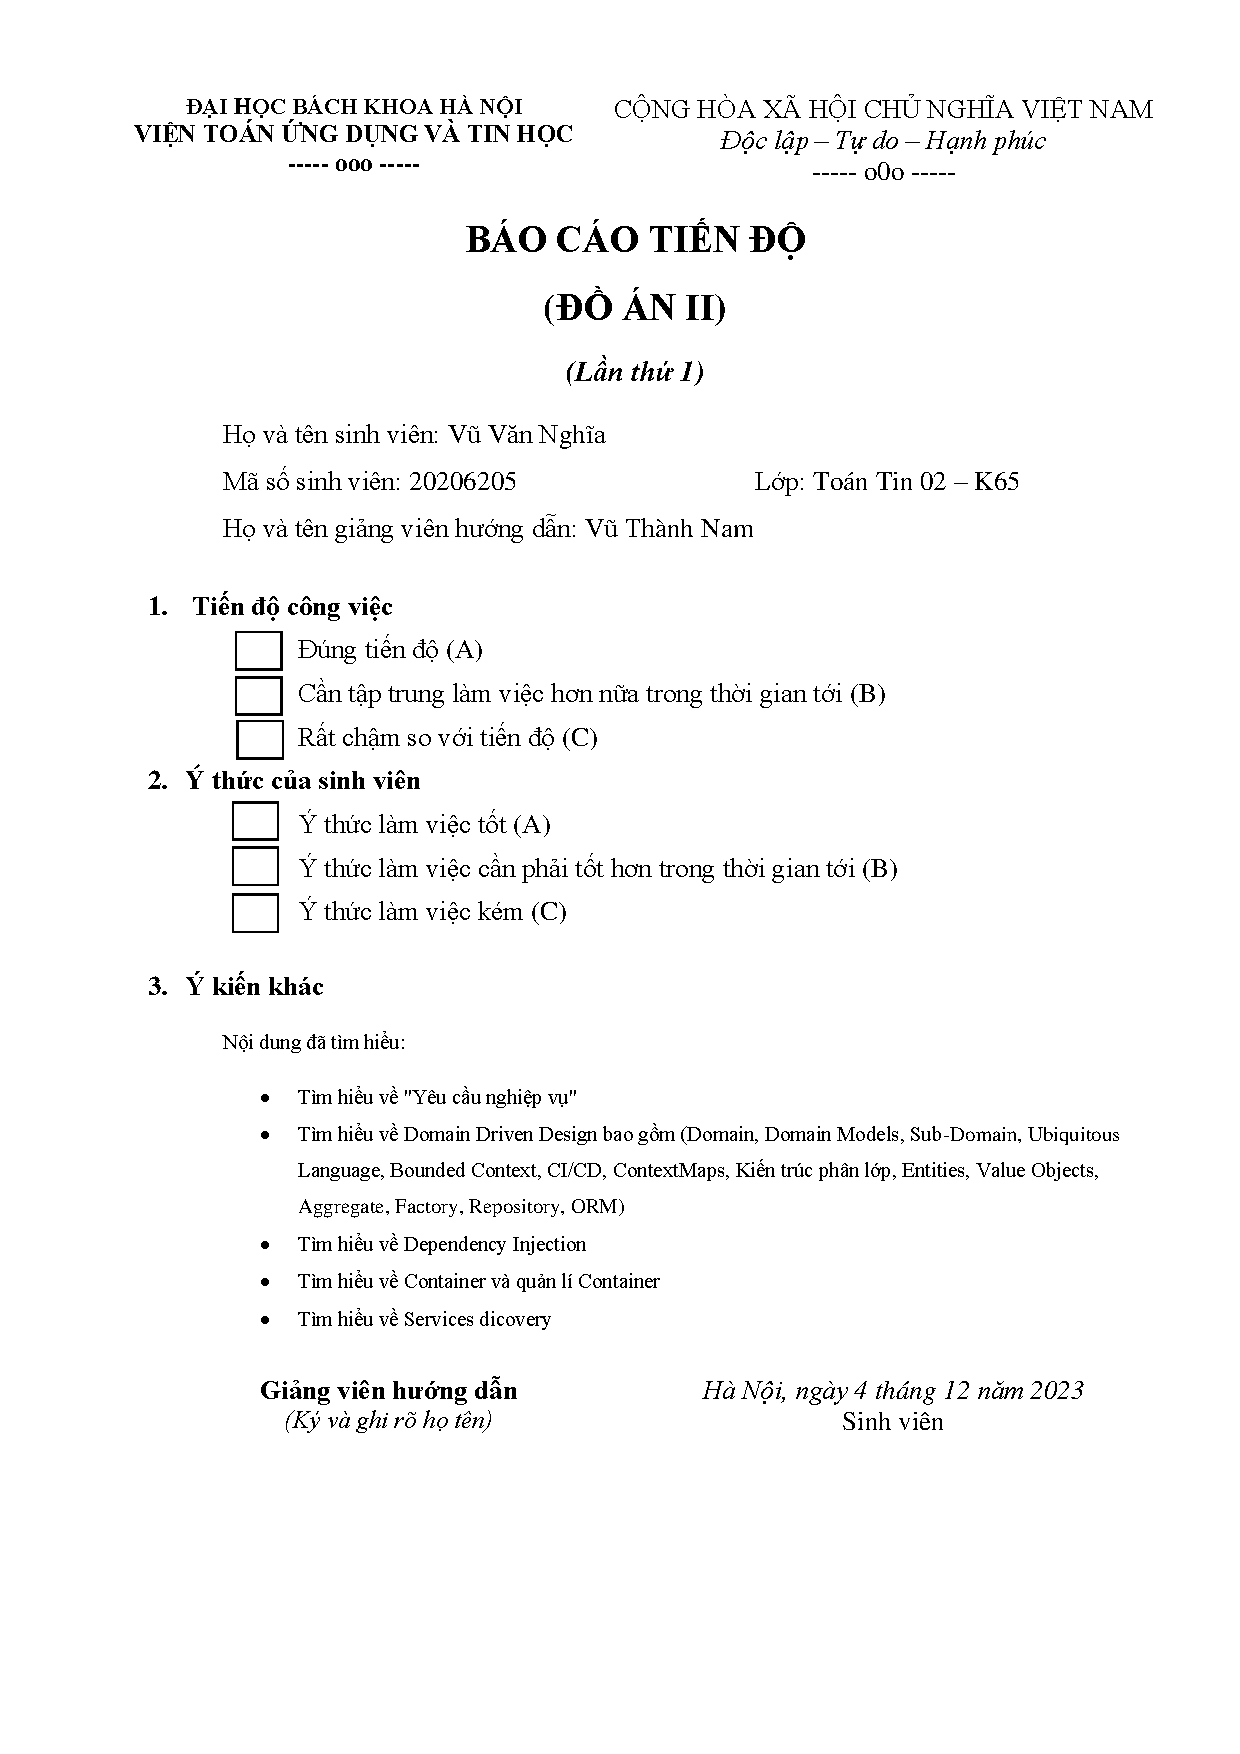
\includepdf[pages = -]{contents/bao_cao_tien_do_1.pdf}
% 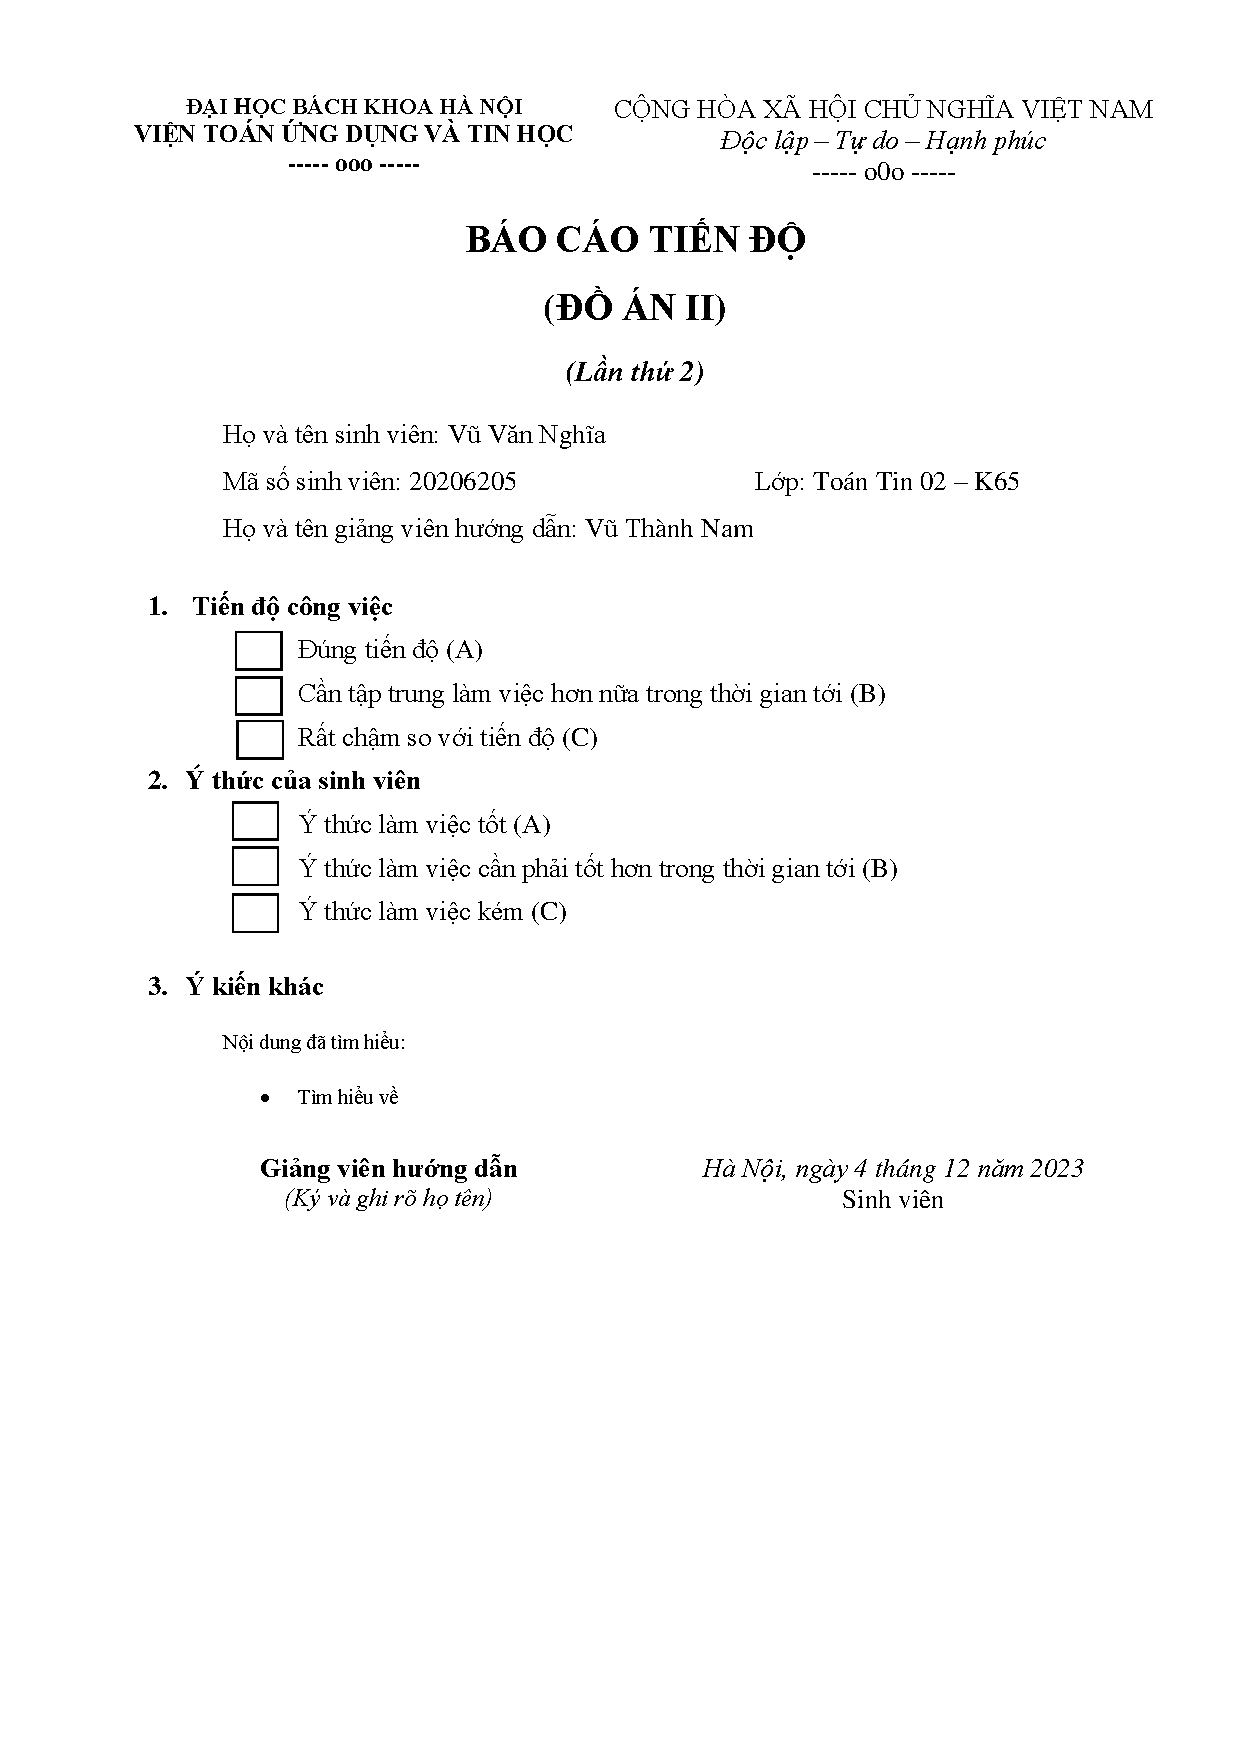
\includepdf[pages = -]{contents/bao_cao_tien_do_2.pdf}
% \newpage
\renewcommand*\contentsname{\centering MỤC LỤC}
\tableofcontents
\newpage


% \newpage

\section*{\centering LỜI CẢM ƠN}

\addcontentsline{toc}{section}{LỜI CẢM ƠN}

\newpage


% \newpage

\section*{\centering LỜI MỞ ĐẦU}

\addcontentsline{toc}{section}{LỜI MỞ ĐẦU}

\newpage
% \newpage
\section*{\centering TÓM TẮT NỘI DUNG ĐỒ ÁN}
\addcontentsline{toc}{section}{TÓM TẮT NỘI DUNG ĐỒ ÁN}
\newpage
% \newpage
\section*{\centering ĐÁNH GIÁ VÀ THẢO LUẬN}
\addcontentsline{toc}{section}{ĐÁNH GIÁ VÀ THẢO LUẬN}
\newpage
\subsubsection{xxxxxxx}
\newpage
\begin{center}
{\bfseries NHẬN XÉT CỦA GIẢNG VIÊN HƯỚNG DẪN}
\end{center}
1.	Mục đích và nội dung của đồ án:

\vspace{4ex} % Thêm khoảng cách dọc

2.	Kết quả đạt được:

3.	Ý thức làm việc của sinh viên:

Hà Nội, \today

\textbf{Giảng viên hướng dẫn}

\textit{(Ký và ghi rõ họ tên)}

\newpage


\end{document} % kết thúc

% \section{Danh sách bảng}
% \section{Danh sách hình ảnh}
% \section{Danh sách mã nguồn}

% \section{Danh sách các cụm từ viết tắt}
% \newpage
\section*{\centering DANH SÁCH CÁC CỤM TỪ VIẾT TẮT}
\addcontentsline{toc}{section}{DANH SÁCH CÁC CỤM TỪ VIẾT TẮT}

% @sau

\begin{table}[h]
\centering
\begin{tabular}{|c|c|c|c|}
\hline
STT & Từ viết tắt & Từ viết đầy đủ & Mô tả \\
\hline
Dong1 & Dong1 & Cot1 & Cot2 \\
\hline
Dong2 & Dong2 & Cot1 & Cot2 \\
\hline
\end{tabular}
\caption{ViDuBangThuong}
\end{table}

\newpage

% API; Application Programming Interface; Giao diện lập trình ứng dụng
% CI/CD; Continuous Integration (CI) and Continuous Delivery (CD) ; Quá trình tích hợp và chuyển giao liên tục
% thiết kế hướng miền ; thiết kế hướng miền; Kỹ thuật thiết kế theo hướng miền
% DI; Dependency Injection; Cơ chế tiêm sự phụ thuộc giữa các đối tượng
% HTTP; Hypertext Transfer Protocol; Giao thức truyền tải siêu văn bản
% JSON; JavaScript Object Notation; Một kiểu dữ liệu mở rộng của JavaScript
% ORM; Object Relational Mapping; Một kỹ thuật ánh xạ các đối tượng lập trình với từng bảng trong CSDL quan hệ
% Cơ sở dữ liệu ; CSDL ;
% Tạo (Create), Đọc (Read), Sửa (Update), Xóa (Delete) ; CRUD ;
% Kubernetes ; K8s ; kubernetes
% Số điện thoại ; SĐT ;
% UML
% MVC; Model View Controller; Một mẫu thiết kế ứng dụng
% SQL

SOA; Service Oriented Architecture; Kiến trúc hướng dịch vụ
SOAP; Simple Object Access Protocol; Một giao thức để truy cập dịch vụ web
SPA; Single Page Application; Kiểu ứng dụng một trang
REST; Representational State Transfer; Một tiêu chuẩn thiết kế các API sử dụng cho các dịch vụ web
URL; Uniform Resource Locator ; Địa chỉ định vị tài nguyên trên Internet
XML; Extensible Markup Language; Ngôn ngữ đánh dấu mở rộng

% TCT ; TCT ;
Người nộp thuế ; NNT ;
Mã số thuế ; MST ;
Hóa đơn điện tử ; HĐĐT ;
Cơ quan thuế ; CQT ;
Công nghệ thông tin ; CNTT ;



% \section{Danh sách các thuật ngữ}
% % STT; Tiếng Anh; Tiếng Việt
% @sau

% kiến trúc nguyên khối, kiến trúc nguyên khối
% kiến trúc nguyên khối, kiến trúc nguyên khối
% kiến trúc vi dịch, kiến trúc vi dịch
% kiến trúc vi dịch, kiến trúc vi dịch
% kiến trúc vi dịch, kiến trúc vi dịch
% kiến trúc vi dịch, kiến trúc vi dịch
% thiết kế hướng miền, thiết kế hướng miền
% thiết kế hướng miền, thiết kế hướng miền

1 thiết kế hướng miền
Thiết kế hướng lĩnh vực
2 Domain (không dịch)
3 Abstraction Trừu tượng
4 chuyên gia ngành
% \subsubsection{xxxxxxx}
% \newpage
\begin{center}
{\bfseries NHẬN XÉT CỦA GIẢNG VIÊN HƯỚNG DẪN}
\end{center}
1.	Mục đích và nội dung của đồ án:

\vspace{4ex} % Thêm khoảng cách dọc

2.	Kết quả đạt được:

3.	Ý thức làm việc của sinh viên:

Hà Nội, \today

\textbf{Giảng viên hướng dẫn}

\textit{(Ký và ghi rõ họ tên)}

\newpage


% \subsubsection{xxxxxxx}
% \newpage
\begin{center}
{\bfseries NHẬN XÉT CỦA GIẢNG VIÊN HƯỚNG DẪN}
\end{center}
1.	Mục đích và nội dung của đồ án:

\vspace{4ex} % Thêm khoảng cách dọc

2.	Kết quả đạt được:

3.	Ý thức làm việc của sinh viên:

Hà Nội, \today

\textbf{Giảng viên hướng dẫn}

\textit{(Ký và ghi rõ họ tên)}

\newpage


%%%%%%%%%%%%%%%%%%%%%%%%%%%%%%%%%%%%%
\end{document} % kết thúc